\documentclass[12pt,a4paper]{article}

\usepackage[T2A]{fontenc}
\usepackage[utf8]{inputenc}
\usepackage[russian]{babel}
\usepackage{amsmath,amssymb}
\usepackage{graphicx}
\usepackage{booktabs}
\usepackage{geometry}
\geometry{margin=2.4cm}
\usepackage{tikz}
\usetikzlibrary{arrows.meta,positioning,shapes.geometric}
\usepackage{float}
\usepackage{caption}
\captionsetup{labelsep=endash}
\usepackage{hyperref}
\hypersetup{colorlinks=true,linkcolor=black,urlcolor=blue}

\title{Лабораторная работа №\,3\\ \large Многокритериальная оптимизация: собственная реализация NSGA-II (трек A)}
\author{Панов Артемий, Б24-527}
\date{2026 г.}

\begin{document}
\maketitle

\section{Постановка задачи и индивидуальный вариант}

Требуется решить многокритериальную задачу распределения задач по
исполнителям по трём критериям (срок, дисбаланс нагрузки, стоимость)
взятой из трека A: собственная реализация NSGA-II без библиотечных
реализаций.

Индивидуальные параметры: $N = 18$, $Q = 2$ (группа 527), $Y = 26$. Номер
варианта:
\[
V = 1 + \big((17N + 7Q + Y) \bmod 20\big) = 1 + (346 \bmod 20) = 7.
\]

\textbf{Вариант 7, трек A} --- распределение задач по исполнителям с
тремя критериями; метод --- NSGA-II (недоминируемая сортировка, расстояние
до скопления, элитизм через объединённый пул, внешний архив).

\section{Формальная модель и данные}

Есть $N = 30$ задач с трудоёмкостями $w_i > 0$ и $M = 6$ исполнителей с
производительностью $p_j$ (объём в час) и ставкой $r_j$ (руб/час).
Назначение $x_i \in \{0, \dots, 5\}$ для каждой задачи. Длительность работ
исполнителя $j$:
\[
\ell_j = \sum_{i:\,x_i=j} \frac{w_i}{p_j}.
\]

Критерии (все минимизируются):
\begin{align}
T(x) &= \max_j \ell_j \quad \text{(срок, makespan)}; \\
I(x) &= \frac{\max_j \ell_j - \min_j \ell_j}{\mathrm{mean}_j \ell_j}
\quad \text{(относительный дисбаланс)}; \\
C(x) &= \sum_{i} \frac{w_i}{p_{x_i}} \cdot r_{x_i}
\quad \text{(стоимость обработки)}.
\end{align}

Экземпляр --- синтетический, генерируется с фиксированным зерном
$\text{seed} = 747$: трудоёмкости $w_i \sim \mathrm{U}(1, 10)$,
производительности $p = (0{,}5;\,0{,}7;\,1{,}0;\,1{,}3;\,1{,}6;\,2{,}0)$,
ставки $r = (15;\,20;\,28;\,40;\,55;\,80)$ руб/час. Быстрые исполнители
заметно дороже --- это источник конфликта критериев (срок против
стоимости).

\section{Представление особи}

Особь --- целочисленный вектор $x = (x_1, \dots, x_{30})$,
$x_i \in \{0, \dots, 5\}$: элемент $i$ --- исполнитель задачи $i$ (та же
структура, что в лабораторной №\,2; здесь ограничение ёмкости снято,
в комплект критериев добавлены дисбаланс и стоимость). Декодирование
тривиально.

\section{Алгоритм NSGA-II (собственная реализация)}

Схема --- на рис.~\ref{fig:nsga}, параметры --- в
таблице~\ref{tab:params}. Используются только собственные реализации
недоминируемой сортировки, расстояния до скопления и отбора.

\begin{figure}[H]
\centering
\resizebox{\textwidth}{!}{%
\begin{tikzpicture}[
  node distance=0.45cm,
  box/.style={draw, rounded corners=2pt, align=center, minimum width=8.2cm,
              minimum height=0.85cm, font=\small},
  dec/.style={draw, diamond, aspect=2.6, align=center, font=\small, inner sep=1pt},
  arr/.style={-{Stealth[length=2.5mm]}, thick}]
\node[box] (init) {инициализация: 100 особей, равномерные назначения};
\node[box, below=of init] (eval) {оценка: вектор критериев (T, I, C)};
\node[dec, below=of eval, yshift=-0.1cm] (stop) {бюджет $2\cdot10^4$ исчерпан?};
\node[box, below=of stop, yshift=-0.3cm] (rank) {недоминируемая сортировка: ранг + расстояние до скопления};
\node[box, below=of rank] (sel) {турнирная селекция по (ранг, скопление)};
\node[box, below=of sel] (cross) {равномерный кроссовер ($p_c = 0{,}9$)};
\node[box, below=of cross] (mut) {мутация: переназначение гена ($p_m = 0{,}05$ на ген)};
\node[box, below=of mut] (pool) {элитизм: объединённый пул «родители + потомки»};
\node[box, right=2.6cm of stop] (end) {конец: финальный фронт Парето};
\draw[arr] (init) -- (eval);
\draw[arr] (eval) -- (stop);
\draw[arr] (stop) -- node[left, font=\small]{нет} (rank);
\draw[arr] (rank) -- (sel);
\draw[arr] (sel) -- (cross);
\draw[arr] (cross) -- (mut);
\draw[arr] (mut) -- (pool);
\draw[arr] (pool.west) -| ++(-1.8,0) |- (eval.west);
\draw[arr] (stop) -- node[above, font=\small]{да} (end);
\end{tikzpicture}}
\caption{Блок-схема NSGA-II}
\label{fig:nsga}
\end{figure}

\begin{table}[H]
\centering
\small
\caption{Параметры NSGA-II}
\label{tab:params}
\begin{tabular}{ll}
\toprule
Параметр & Значение \\
\midrule
Размер популяции & 100 ($\ge 30$ по заданию) \\
Селекция & турнирная по паре (ранг, затем расстояние до скопления) \\
Рекомбинация & равномерный кроссовер, $p_c = 0{,}9$ \\
Мутация & переназначение гена случайному исполнителю, $p_m = 0{,}05$ на ген \\
Сохранение лучших & элитизм через объединённый пул (ранг + скопление) \\
Критерий остановки & бюджет $20\,000$ вычислений вектора критериев \\
Серия & 30 независимых запусков, $\text{seed} = 9000 + 19i$ \\
\bottomrule
\end{tabular}
\end{table}

\textbf{Новые относительно ЛР1--2 механизмы} (требование трека A):
недоминируемая сортировка (ранги), расстояние до скопления
(crowding distance), внешний архив недоминируемых решений (объединение
фронтов серии).

\textbf{Турнир по (ранг, скопление)}: выигрывает меньший ранг; при
равенстве --- большее расстояние до скопления. Расстояние до скопления:
крайним точкам каждого критерия --- бесконечность.

\textbf{Гиперобъём (HV)}. Для оценки качества серии используется точный
3D-гиперобъём методом слайсинга: по уровням первого критерия площадь
сечения --- точный 2D HV активных точек. Опорная точка ---
$\mathrm{ref} = 1{,}05 \times \max$ по объединённому архиву серии.
Корректность проверена на заранее посчитанном примере (HV = 7).

\section{Обоснование выбора операторов}

Структура задачи: назначения --- целочисленный вектор по задачам. Отсюда:
\begin{itemize}
\item \textbf{равномерный кроссовер} --- осмысленно смешивает назначения
  по отдельным задачам (в ЛР\,2 показал результаты наравне с
  одноточечным);
\item \textbf{мутация по гену} --- мелкая варьирующая операция для
  векторов назначений;
\item \textbf{ранг + скопление} --- стабилизирует фронт как множество,
  не схлопывая его в одну точку;
\item \textbf{элитизм через пул} --- гарантирует монотонное приближение
  фронта поколение к поколению.
\end{itemize}

\section{Методология эксперимента}

Три эксперимента при фиксированном бюджете $20\,000$ вычислений:
\begin{enumerate}
\item \textbf{серия NSGA-II}: 30 запусков, зерна $9000 + 19i$; финальные
  фронты объединяются в архив (2997 точек), из которого отбираются только
  недоминируемые --- общий фронт серии; по серии считается гиперобъём
  каждого финального фронта при общей опорной точке;
\item \textbf{сравнение со взвешенной суммой}: одно-критериальный ГА со
  скалярным фитнесом $g(x) = \sum_k \lambda_k \hat F_k(x)$, веса
  $\lambda$ --- распределение Дирихле (свои для запуска); сравнение по
  доминируемости и гиперобъёму при той же опорной точке;
\item \textbf{характерные решения}: из общего фронта --- экстремальные по
  каждому критерию и «колено» (ближайшая к идеалу после нормировки); две
  базовые линии: жадная LPT-диспетчеризация и назначение каждой задачи
  самому дешёвому исполнителю.
\end{enumerate}

Метрики серии: лучшее, среднее, медиана, стандартное отклонение, худшее
значение гиперобъёма.

\section{Результаты: серия NSGA-II и общий фронт}

\begin{table}[H]
\centering
\small
\caption{Гиперобъём по 30 запускам NSGA-II (общая опорная точка)}
\label{tab:hv}
\begin{tabular}{lccccc}
\toprule
Метрика & Лучший (max) & Среднее & Медиана & Станд. откл. & Худший (min) \\
\midrule
HV & 718\,299 & 711\,298 & 712\,028 & 4\,349 & 702\,669 \\
\bottomrule
\end{tabular}
\end{table}

Размеры финальных фронтов --- около 100 точек (вся финальная популяция
недоминируема --- отсюда массивный внешний архив). Разброс HV на серии
$\mathrm{std}/\mathrm{mean} \approx 0{,}6\%$ --- серия устойчива к
инициализации (таблица~\ref{tab:hv}, рис.~\ref{fig:hv}).

\begin{figure}[H]
\centering
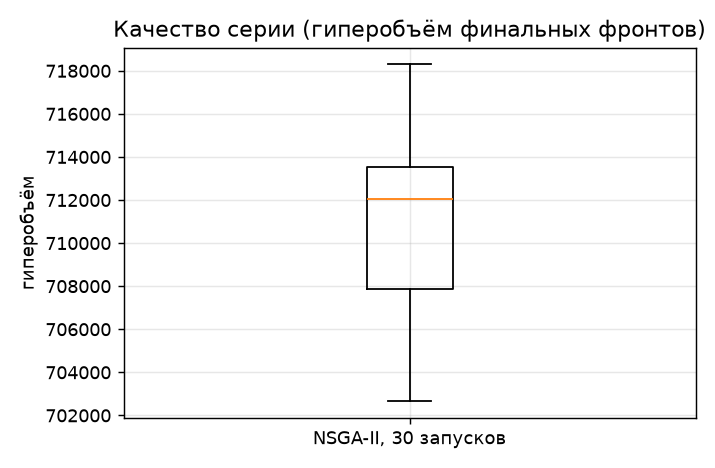
\includegraphics[width=0.6\textwidth]{figures/hv_boxplot.png}
\caption{Качество серии (гиперобъём финальных фронтов, 30 запусков)}
\label{fig:hv}
\end{figure}

Общий фронт серии --- 810 недоминируемых точек из 2997 в архиве
(рис.~\ref{fig:front}). Заметим, что HV общего фронта ($734\,499$) выше
HV любого отдельного запуска (максимум $718\,299$): это ожидаемо, так как
общий фронт является объединением финальных фронтов и содержит больше
недоминируемых точек.

\begin{figure}[H]
\centering
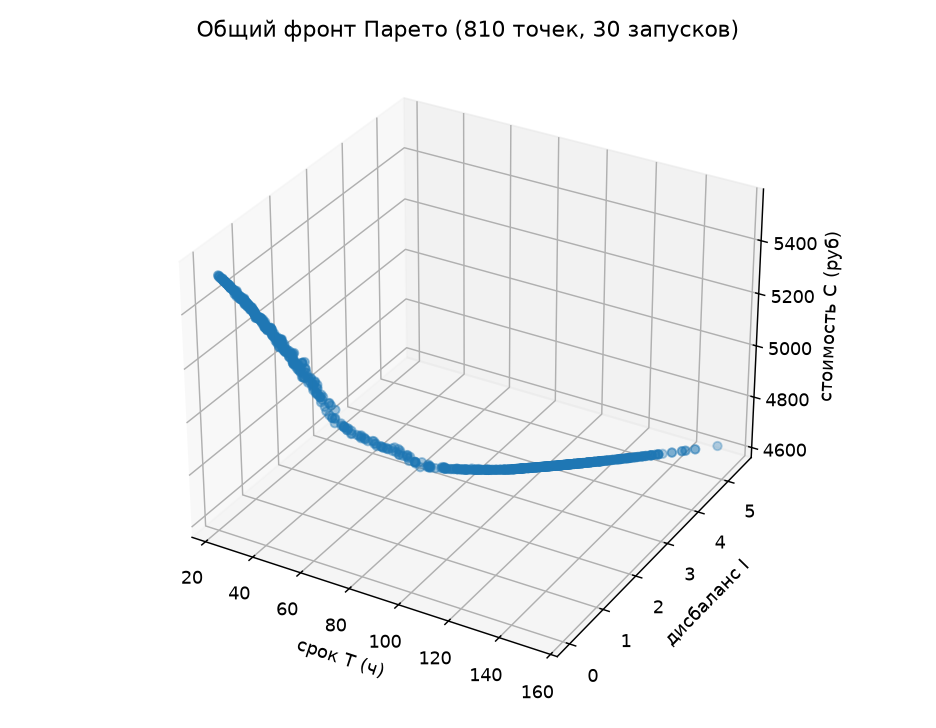
\includegraphics[width=0.72\textwidth]{figures/pareto_front_3d.png}
\caption{Общий фронт Парето (810 точек, 30 запусков)}
\label{fig:front}
\end{figure}

\begin{figure}[H]
\centering
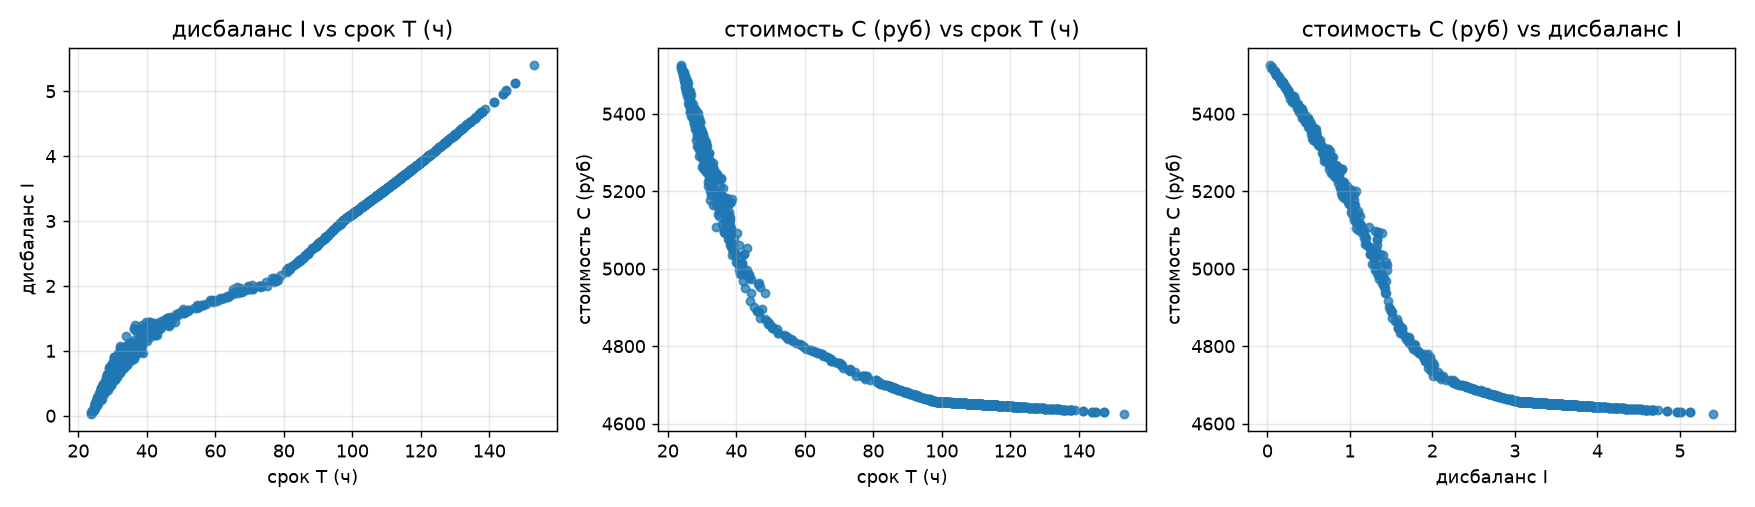
\includegraphics[width=0.98\textwidth]{figures/pareto_projections.png}
\caption{Попарные проекции общего фронта Парето}
\label{fig:proj}
\end{figure}

Фронт покрывает содержательные компромиссы (рис.~\ref{fig:proj}): слева в
проекции «срок--дисбаланс» --- быстрые сбалансированные назначения
(срок 23{,}7, дисбаланс 0{,}03); справа в проекции «стоимость» ---
дешёвые назначения на медленных исполнителях (стоимость 4626 при сроке
153).

\section{Результаты: сравнение со взвешенной суммой}

\begin{table}[H]
\centering
\small
\caption{NSGA-II против одно-критериального ГА на взвешенной сумме
(30 случайных векторов весов; та же опорная точка HV)}
\label{tab:weighted}
\begin{tabular}{lcc}
\toprule
Метод & Гиперобъём & Доля доминируемых точек \\
\midrule
NSGA-II, общий фронт (810 точек) & $\mathbf{734\,499}$ & --- \\
Взвешенная сумма (30 точек) & 648\,523 & 50\% \\
\bottomrule
\end{tabular}
\end{table}

\begin{figure}[H]
\centering
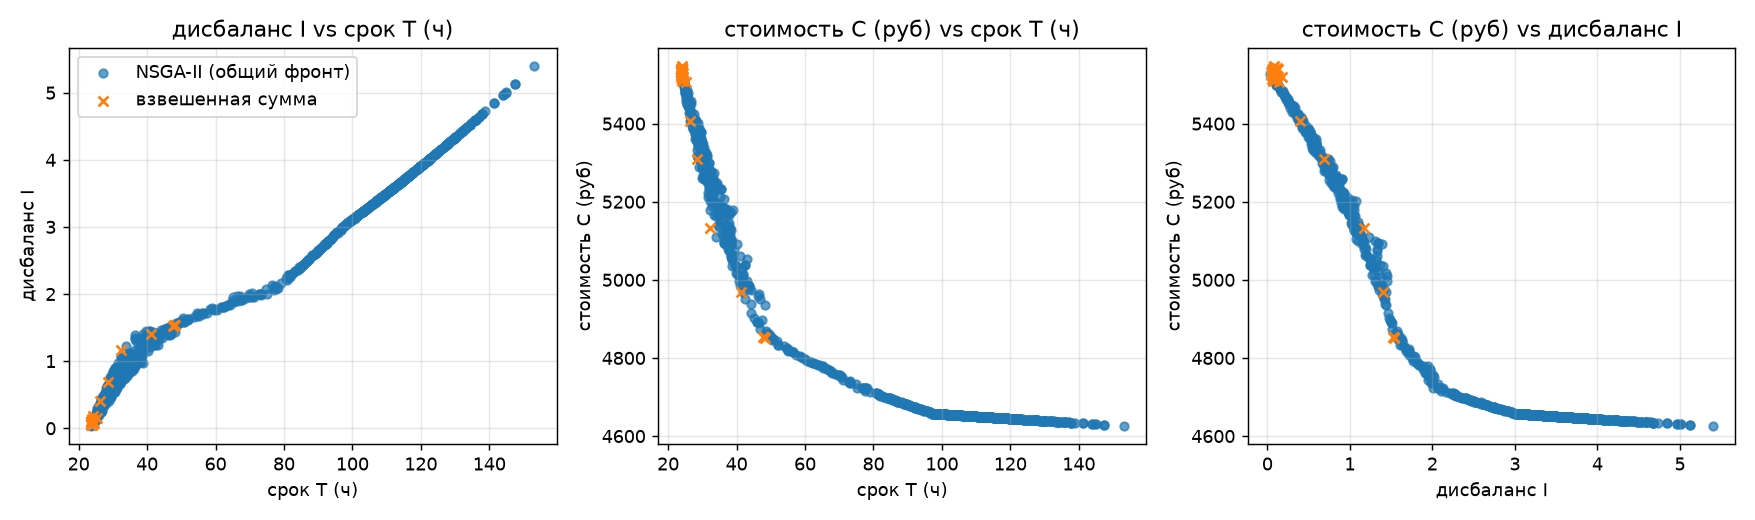
\includegraphics[width=0.98\textwidth]{figures/pareto_weighted.png}
\caption{Общий фронт NSGA-II против точек взвешенной суммы
(три попарные проекции)}
\label{fig:weighted}
\end{figure}

Сравнение на равном бюджете $2\cdot 10^4$ вычислений (таблица~\ref{tab:weighted},
рис.~\ref{fig:weighted}): половина точек взвешенной суммы доминируется
общим фронтом NSGA-II, а гиперобъём NSGA-II заметно выше
($734\,499 > 648\,523$). Причина: случайные веса $\lambda$ редко
попадают в углы фронта, а одно-критериальный ГА не удерживает разнообразие
фронта --- он сходится в одну точечную оценку.

\section{Результаты: характерные решения и базовые линии}

\begin{table}[H]
\centering
\small
\caption{Характерные решения общего фронта и базовые линии}
\label{tab:reps}
\begin{tabular}{lccc}
\toprule
Решение & Срок $T$ (ч) & Дисбаланс $I$ & Стоимость $C$ (руб) \\
\midrule
быстрое (min срок) & $\mathbf{23{,}695}$ & $\mathbf{0{,}0323}$ & 5\,526 \\
сбалансированное (min дисбаланс) & 23{,}695 & 0{,}0323 & 5\,526 \\
дешёвое (min стоимость) & 153{,}152 & 5{,}4047 & 4\,626 \\
колено (ближ. к идеалу) & 23{,}695 & 0{,}0323 & 5\,526 \\
\midrule
LPT (жадная эвристика) & 24{,}166 & 0{,}0568 & 5\,522 \\
дешёвая эвристика & 164{,}960 & 6{,}0000 & 4\,619 \\
\bottomrule
\end{tabular}
\end{table}

Сравним LPT с точкой «быстрое» из общего фронта. По сроку и дисбалансу
фронт лучше: $23{,}695 < 24{,}166$ и $0{,}0323 < 0{,}0568$. По стоимости
LPT формально немного лучше: $5\,522 < 5\,526$, но разница составляет
около $0{,}07\%$, то есть пренебрежимо мала. Поэтому можно сказать, что
фронт практически доминирует жадную LPT-диспетчеризацию, уступая ей лишь
в пределах малой вариации по стоимости.

Детерминированная «дешёвая эвристика» (каждую задачу --- самому дешёвому
исполнителю) почти совпадает с краем фронта по стоимости
($4\,619$ против $4\,626$ --- разница около $0{,}15\%$), но даёт заметно
худший дисбаланс $6{,}0$. Таблица~\ref{tab:reps} даёт содержательную
интерпретацию краёв фронта: «быстрое» соответствует экстремуму по сроку,
«дешёвое» --- экстремуму по стоимости; «сбалансированное» совпадает с
«быстрым», поскольку в этой задаче минимизация срока и дисбаланса
действуют в одном направлении.

\section{Оценка результата и выводы}

Полученный результат --- \textbf{хороший} для поставленной задачи: во
всех 30 запусках NSGA-II без библиотек восстановлен устойчивый фронт
Парето (разброс HV $\approx 0{,}6\%$), общий фронт содержит 810
недоминируемых точек и доминирует половину точек взвешенной суммы при
равном бюджете.

Выводы:
\begin{enumerate}
\item собственная реализация NSGA-II (недоминируемая сортировка,
  расстояние до скопления, элитизм через объединённый пул) устойчиво
  восстанавливает плотный фронт Парето для трёх критериев;
\item взвешенная сумма критериев проигрывает: 50\% её точек
  доминируются общим фронтом NSGA-II, а гиперобъём выше
  ($734\,499 > 648\,523$) при равном бюджете;
\item жадная LPT-диспетчеризация практически доминируется фронтом:
  точка «быстрое» лучше по сроку и дисбалансу, а по стоимости разница
  составляет около $0{,}07\%$; жадная «дешёвая» эвристика --- почти
  край фронта по стоимости, но с существенно худшим дисбалансом;
\item гиперобъём --- рабочая скалярная метрика серии; бюджет измеряется
  в вычислениях функции у обоих подходов (честное сравнение);
\item точный метод слайсинга для 3D HV проверен на контрольном примере.
\end{enumerate}

\section*{Состав материалов}

\begin{itemize}
\item \texttt{lab3.ipynb} --- ноутбук с полным кодом и всеми
  экспериментами (выполнен, с результатами);
\item \texttt{report.tex}, \texttt{report.pdf} --- настоящий отчёт;
\item \texttt{figures/hv\_boxplot.png} --- гиперобъём серии;
\item \texttt{figures/pareto\_front\_3d.png} --- фронт Парето 3D;
\item \texttt{figures/pareto\_projections.png} --- попарные проекции;
\item \texttt{figures/pareto\_weighted.png} --- сравнение со взвешенной
  суммой;
\item \texttt{results/runs\_nsga2.csv} --- запуски серии;
\item \texttt{results/summary\_hv.csv} --- сводный HV;
\item \texttt{results/pooled\_front.csv} --- общий фронт (810 точек);
\item \texttt{results/weighted\_sum.csv},
  \texttt{results/summary\_weighted.csv} --- сравнение;
\item \texttt{results/representative\_solutions.csv} --- характерные
  решения и базовые линии;
\item \texttt{README.md} --- инструкция по запуску.
\end{itemize}

\end{document}